\section{Orbit Analysis}
This section is about the trade-off for the orbit characteristics. First the orbit design options are compared with the killer requirements. After that the section is split into two major pieces, one containing special orbits and the altitude of the orbit, and another one that considers the swarm in greater detail.
\label{AnalOrb}

\subsection{Eliminating the obvious losers}
\label{pruneOrbit}
The orbits of the satellites are determined by the characteristics of the emitter and receivers. Because the payload uses a low power laser this means that the orbits will have to be \ac{LEO} in order for the receivers to receive enough, or any, photons. The resulting design option tree can be found in figure \ref{fig:pruneOrbit}, on page \pageref{fig:pruneOrbit}. Further pruning is not possible without a detailed analysis of the remaining options, which is done in the following section.

\begin{figure}[b]
\centering
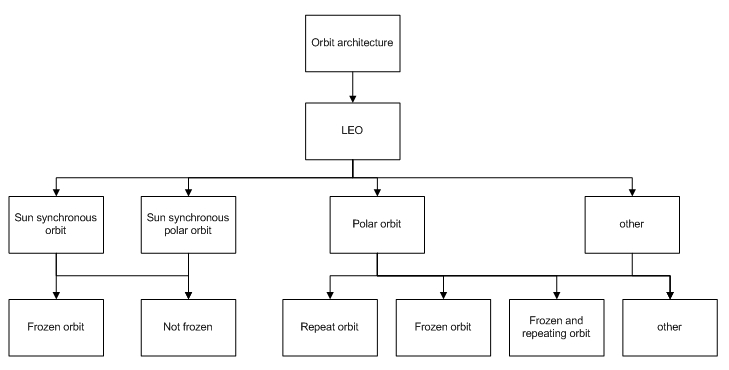
\includegraphics[width=1.0\textwidth, angle=0]{chapters/img/PrunedOrbit.jpg}
\label{fig:pruneOrbit}
\caption{Pruned design option tree for the orbit characteristics}
\end{figure}

\subsection{Analysis of the remaining options}
\label{AnalSpOrb}

In subsection \ref{pruneOrbit} the design option tree was pruned by comparing the orbit altitudes with the altitude requirement that follows from the payload. As a result the \acs{MEO}, \acs{GEO} and \acs{HEO} were eliminated. The remaining options will now be analyzed.

No trade-off table will be made for this section. Instead the four special types of orbits seen in figure \ref{fig:pruneOrbit} will be compared with the mission requirements and eliminated separately. The four orbit types are polar orbit, sun synchronous orbit, repeating ground track orbit and frozen orbit. After that another section will investigate preliminary parameter values for the final design option.

\subsubsection{Polar orbit}
An orbit is a polar orbit if the orbit inclination is exactly 90 degrees. However, it is not uncommon for an orbit to be classified as a polar orbit if the inclination is close to 90 degrees. For the case of the laser swarm it is assumed that an orbit is a polar orbit if the inclination is between 80 and 100 degrees.

The laser swarm should be able to observe any region on Earth, including the poles. As such the final orbit design option has to be a polar orbit.

\subsubsection{Sun Synchronous orbit}
A sun synchronous orbit is an orbit that uses the fact the Earth is not a perfect sphere, thus allowing a satellite to orbit the planet in such a way that the plane of the orbit rotates around the Earth's polar axis exactly once a year. Thus fixing the satellite's orbital plane with respect to the sun vector.

While providing useful conditions, it is not required for the swarm to use this kind of orbit unless certain power or lighting requirements have to be met, as the simulation has shown this to be unnecessary the final orbit design will not be sun synchronous.

\subsubsection{Repeating ground track orbit}
Repeating ground track orbits, or in short repeat orbits, are orbits that repeat after a predefined amount of time after the satellite has traveled an integral amount of revolutions. This type of orbit is useful as it allows one to revisit the same area, thus making it possible to view an area at different times. Which may provide useful information on variables that change over time.
To determine if it is an option for the laser swarm, a calculation is made to check whether the constellation can actually see the entire Earth in five years.

The Earth circumference is 40.000 [km], now assuming a footprint of 100 [m] this means that it will take $40.000.000/(2*100)=200.000$ revolutions to see all of this 40.000 [km]. Note that the factor 2 arises from the Earth being a sphere, thus the satellite sees the equator twice during a single revolution. Assuming a very low orbit of 300 [km] with a period of 90 [minutes](\cite{larson}) the time taken for these 200.000 revolutions is $200.000*90=1.800.000$ [minutes]. This is equal to approximately 34 years.

From the previous calculation it is clear that a repeat orbit is undesirable as it would mean even less of the Earth surface is covered in the 5 year lifetime. Also the type of sensor used, a \ac{SPAD}, can oversample an area when viewing it.

\subsubsection{Frozen orbit}
A frozen orbit is an orbit for which the time rate of change of the inclination, eccentricity and argument of perigee are equal or close to zero. These conditions are favorable as they reduce the amount of stationkeeping, thus reducing the need for attitude control. This in turn means less fuel which makes the structure lighter, etc.
This setup is very advantageous to the laser swarm as the formation has to remain the same, and because many satellites have to be launched even a small weigh reduction will have significant effect on the total weight. For these reasons the frozen orbit is also a design choice.

\subsection{Preliminary Orbit Parameters}
The resulting design choice for the laser swarm is a frozen polar orbit. In this section some of preliminary values for the six orbital elements will be determined, using the constraints given by \ref{constraints}.

\begin{equation}
\frac{{d\omega }}{{dt}} = 0,\quad \frac{{di }}{{dt}} = 0,\quad \frac{{de }}{{dt}} = 0,\quad 80\ [deg] \leq i \leq 100\ [deg]
\label{constraints}
\end{equation}

The equations used to make an orbit a frozen orbit are given by \ref{FrozenEcc} for the time derivative of the eccentricity, \ref{FrozenInc} for the time rate of change of the eccentricity and finally \ref{FrozenArg} for the time rate of change of the argument of perigee. Note that \ref{FrozenF} is a continuation of \ref{FrozenArg}. The terms n and p in these equations represent the mean motion and semiparameter respectively, and are given by equations \ref{meanMotion} and \ref{p}.

% FROZEN ORBIT

% ..., the constraint equation for the time rate of change of the eccentricity for a frozen orbit
\begin{equation}
\dot e = \frac{3}
{2}\frac{{J_3 r_{eq}^3 }}
{{p^3 }}\left( {1 - e^2 } \right)n\sin i \cdot \cos \omega \left( {\frac{5}
{4}\sin ^2 i - 1} \right) = 0
\label{FrozenEcc}
\end{equation}

% Frozen orbit inclination thing.
\begin{equation}
\frac{{di}}
{{dt}} = \frac{3}
{2}\frac{{J_3 n}}
{{\left( {1 - e^2 } \right)^3 }}\left( {\frac{{R_e }}
{a}} \right)^3 e\cos i \cdot \cos \omega \left( {\frac{5}
{4}\sin ^2 i - 1} \right) = 0
\label{FrozenInc}
\end{equation}

% The constraint equation for the time rate of change of the argument of perigee for a frozen orbit, notice the presence of the J3 term in F
\begin{equation}
\dot \omega  = \frac{{3J_2 n}}
{{\left( {1 - e^2 } \right)^2 }}\left( {\frac{{R_e }}
{a}} \right)^2 \left( {1 - \frac{5}
{4}\sin ^2 i} \right)F
\label{FrozenArg}
\end{equation}

% Arg continued
\begin{equation}
F = 1 + \frac{{J_3 }}
{{2J_2 \left( {1 - e^2 } \right)}}\left( {\frac{{R_e }}
{a}} \right)\left( {\frac{{\sin ^2 i - e^2 \cos ^2 i}}
{{\sin i}}} \right)\frac{{\sin \omega }}
{e}
\label{FrozenF}
\end{equation}

% Mean motion
\begin{equation}
n = \sqrt {\frac{\mu }
{{a^3 }}} 
\label{meanMotion}
\end{equation}

% p
\begin{equation}
p = a\left( {1 - e^2 } \right)
\label{p}
\end{equation}

Before investigating these equations the eccentricity is set equal to zero, the reason for this is that the mirrors or lenses on the satellites do not have to refocus and it allows for easier data handling.
The result is that equation \ref{FrozenInc} is automatically satisfied for any inclination, eccentricity, argument of perigee and semimajor axis. So the orbit is frozen w.r.t. the inclination.

Another effect caused by setting the eccentricity to zero is that the argument of perigee can not be distinguished from another point in the orbit. While it would still indicates the perigee, it is meaningless because the orbit is circular. As such the argument of perigee assumed to be able to take any value and so is set equal to 90 degrees, resulting in $de/dt$ to become equal to zero for any inclination and altitude.

\begin{figure}
\centering
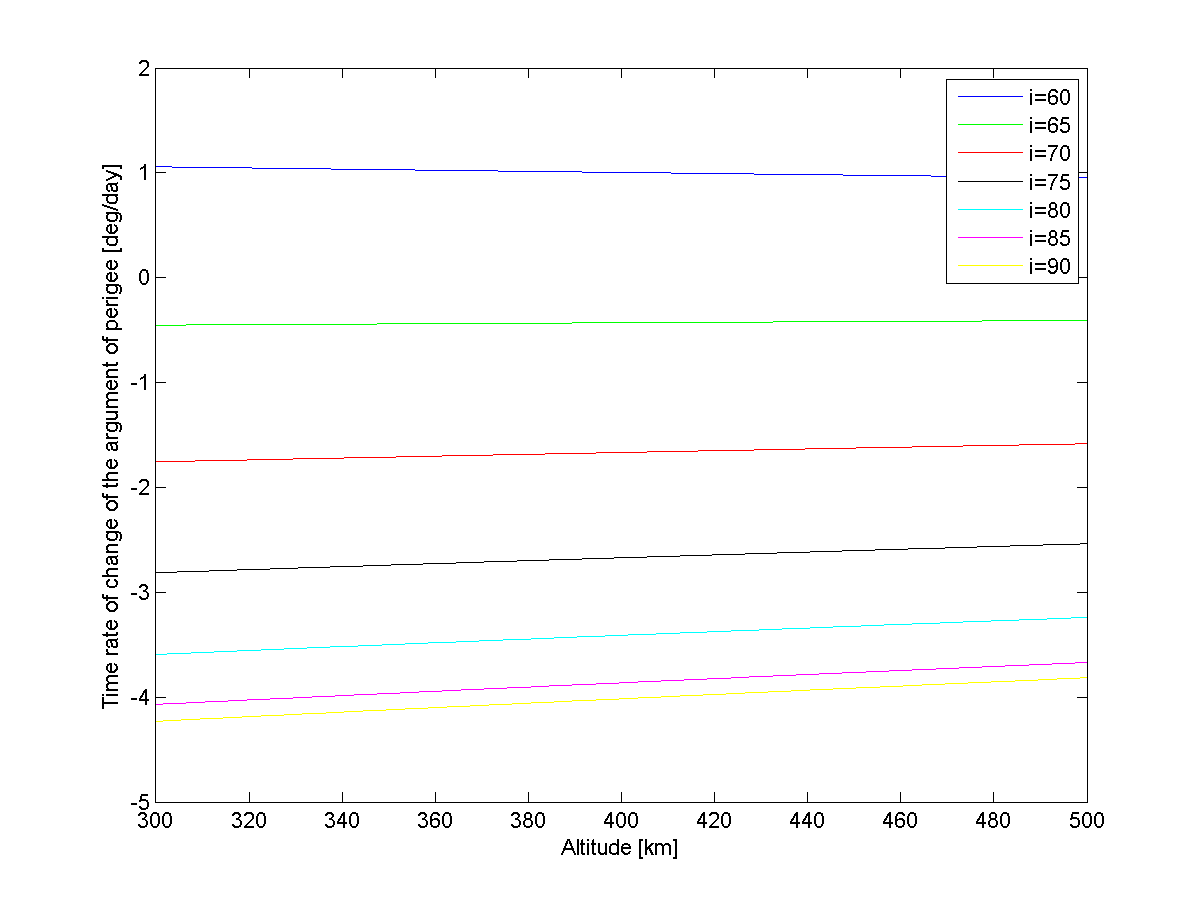
\includegraphics[width=0.8\textwidth, angle=0]{chapters/img/AltVsOmdot.png}
\label{fig:AltVsOmdot}
\caption{$d\omega/dt$ for a range of altitudes and several different inclinations.}
\end{figure}

Figures \ref{fig:AltVsOmdot} shows the only remaining condition for a frozen orbit for several values of inclination. From this figure and equation \ref{FrozenArg} it can be seen that $d\omega/dt$ is equal to zero if the inclination is equal to 63.43 [deg]. However the constraints (\ref{constraints}) indicate this is not a possibility. Figure \ref{fig:AltVsOmdot} shows that $d\omega/dt$ is maximal at 90 degrees inclination, however the difference between i=80 [deg] and i=90[deg] is only 0.5 [deg/day]. As a result the extra 0.5 [deg/day] is considered an acceptable loss compared to the increased coverage provided by the increased inclination. However an inclination of 90 [deg] creates problems with collision avoidance for the swarm, so instead an inclination of 85 [deg] is chosen. This allows for an almost complete coverage and a small decrease in the value of $d\omega/dt$, as seen in figure \ref{fig:AltVsOmdot}. Note that an inclination of 85 [deg] is chosen instead of an inclination of 95 [deg] is that 85 [deg] inclination means the orbit is prograde, which reduces the required $\Delta$V. Equation \ref{FrozenArg} indicates that the rate of change for the argument of perigee is the same.

Summarizing the results so far yields that the inclination is equal to 85 [deg], the eccentricity is equal to 0 [-], and the argument of perigee is equal to 90 [deg].